\renewcommand\thisdir{papers/rtas22a}
\tikzsetfigurename{rtas22a-}
\renewcommand\figdir{\thisdir/figs}

% Commands for this paper
% if the conflict with previously defined commands use \renewcommand
%%%%%%%%%%%%%%%%%%%%%%%%%%%%%%%%%%%%%%%%%%%%%%%%%%%%%%%%%%%%%%%%%%%%%%%%%%%%%%%%
% In this file, only commands are allowed. These commands should be explained to
% greatest possible extent.
%%%%%%%%%%%%%%%%%%%%%%%%%%%%%%%%%%%%%%%%%%%%%%%%%%%%%%%%%%%%%%%%%%%%%%%%%%%%%%%%

% Real-time
\newcommand{\counter}{q}

% Plots
\newcommand{\timeplotheight}{4.9cm}

% Tables
\definecolor{Gray}{gray}{0.9}
\newcolumntype{a}{>{\centering\arraybackslash\columncolor{Gray}}m{0.075\columnwidth}}
\newcolumntype{b}{>{\centering\arraybackslash\columncolor{white}}m{0.075\columnwidth}}

% Set number of bins for aggregated plants histograms
\newcommand{\binsaggregatedhist}[0]{65}

%%% Colors
\definecolor{misscolour}{RGB}{255, 0, 0}
\definecolor{lqrcolour}{RGB}{0,28,255}
\definecolor{lqrnomcolour}{RGB}{0,28,255}
\definecolor{lqgcolour}{RGB}{0,139,0}
\definecolor{lqgnomcolour}{RGB}{0,139,0}
\definecolor{adacolour}{RGB}{239,133,16}


\paper[Deadline-Miss-Adaptive Controller Implementation]{Deadline-Miss-Adaptive Controller Implementation for Real-Time Control Systems}
\authors{Nils Vreman \and Claudio Mandrioli \and Anton Cervin}

\begin{abstract}
    The policy used to implement a control algorithm in a real-time system can significantly affect the quality of control.
    In this paper, we present a method to adapt the controller implementation, with the objective to improve the system's performance under real-time faults.
    Our method compensates for missing state updates by adapting the controller parameters according to the number of consecutively missed deadlines. 
    It extends the state-of-the-art by considering dynamic controllers, which have had limited coverage in previous literature.
    The adaptation mechanism can be precomputed offline, solely based on knowledge about the controller and not on the controlled plant. 
    The approach is indifferent to the control design, as well as to the scheduling policy, and can be automatically realised by the operating system, thus improving the robustness of the control system to intermittent and unexpected real-time faults.
    We develop a stochastic performance analysis method and apply it to both a real plant and numerous simulated plants to evaluate our adaptive controller.
    Complementary to the stochastic analysis, we also do worst-case stability analysis of the resulting system.
    The results confirm the conjuncture that the adaptive controller improves both the performance and robustness in the presence of deadline misses.
\end{abstract}

\vfill
Originally published in IEEE 28th Real-Time and Embedded Technology and Applications Symposium (2022).
The mathematical notation has been unified to match the remainder of the thesis.
Reprinted with permission.
\newpage

\section{Introduction}
\label{sec:intro}
A recent survey on the state of industrial practice in real-time systems showed that a significant fraction of real-time tasks are allowed to miss a finite number of deadlines~\cite{Akesson:2020}.
%
The research community spent years defining and analysing models of tasks that can miss deadlines, from soft real-time systems~\cite{Buttazzo:2005}, to tasks with a skip-factor~\cite{Koren:1995}, from calculating the miss ratio based on execution time probability distributions~\cite{Manolache:2004}, to approximating the deadline miss probability~\cite{vonDerBruggen:2018, Bozhko:2021, vonderBrueggen:2021} for a given system.

One of such models in which tasks may miss deadlines is the weakly-hard task model~\cite{Bernat:2001}. 
Weakly-hard tasks behave according to patterns of hit and missed deadlines that are (mainly) window-based.
The originally proposed constraint models specifies alternatively (for a window of subsequent jobs):
\begin{enumerate*}[label=(\roman*)]
    \item the minimum number of deadlines that are hit,
    \item the minimum number of consecutive deadlines that are hit,
    \item the maximum number of deadlines that may be missed, or
    \item the maximum number of consecutive deadlines that may be missed.
\end{enumerate*}
The third of these models -- often called the $(m,K)$ model -- gained attention in the research community, generating results on scheduling algorithms~\cite{Hamdaoui:1995}, real-time and schedulability analysis~\cite{Sun:2017, Pazzaglia:2021b, Hammadeh:2017}, verification~\cite{Huang:2019b, Behrouzian:2020} and runtime monitoring~\cite{Wu:2020} of constraint satisfaction, derivation of task model parameters~\cite{Xu:2015}, together with applications to domains like telecommunication~\cite{Ahrendts:2018, Huang:2019a} and control systems~\cite{Ramanathan:1999, Pazzaglia:2018, Vreman:2021, Pazzaglia:2021}. 
The fourth model has also proved relevant to perform analyses of the stability of control systems~\cite{Maggio:2020}. 
Furthermore, the relation between weakly-hard constraint types has been partially investigated~\cite{Tu:2007, Wu:2020}.
However, this investigation remains partial as some of the constraints are not connected and their dominance (i.e., the comparison of how strictly does the task model constrain the task execution for different types of constraints) is not assessed.

The practical usefulness of weakly-hard models will remain limited, unless it is possible to build tools to enforce and monitor the satisfaction of weakly-hard constraints for execution platforms.
Many real-time platforms offer the possibility to invoke ``protected'' task executions, ensuring that deadlines are met at the cost of increasing the execution cost.
This is a very simple mechanism to secure that the weakly-hard constraint is satisfied in an execution platform.
However, this requires writing monitoring code, that generates transition points to this protected execution mode when a constraint might otherwise be violated.
Generating this code in a scalable way requires abstracting from the constraint and representing the execution of tasks with compact, but expressive, models.

To date, the literature has focused on the $(m,K)$ constraint, neglecting the others, despite their relevance in application domains such as control~\cite{Maggio:2020, Linsenmayer:2017, Vreman:2021}.
As a result, the mentioned tools and models are not available for all the constraint types.
This paper aims at both solving this problem and answering some open issues, namely:
\begin{enumerate*}[label=(\roman*)]
    \item guaranteeing consecutive deadline hits, and not only following patterns of deadline misses; and
    \item dealing with systems that satisfy multiple weakly-hard constraint simultaneously.
\end{enumerate*}

The first issue comes from the consideration that in practice it may be easier to guarantee that some prescribed job will hit their deadline rather than ensuring that the number of misses follows a given pattern. 
This is the case of the mentioned protected execution environment. 
As an example, mixed-criticality allows the scheduler to raise the criticality level and thus guarantee that the highly-critical tasks meet the corresponding deadlines~\cite{Burns:2013}. 
We can treat the weakly-hard task as highly critical and raise the criticality level when a deadline hit must be enforced. 
Alternatively, we can increase the budget of a reservation-based scheduler~\cite{Casini:2019}.
Despite the fact that guaranteeing hits is often easier than enforcing miss patterns, the first two types of weakly hard tasks, that constrain the number of hits, have not been receiving much attention from the research community.

Furthermore, we would like to analyse tasks that satisfy multiple constraints simultaneously.
Most analysis methods only take into account a single constraint, e.g.,~\cite{Pazzaglia:2018} or~\cite{Maggio:2020} for the stability of control systems.
In some cases, one of the two constraints \emph{dominates} the other, meaning that satisfying the dominant constraint also guarantees the satisfaction of the dominated one. 
But this is not always the case.
Consider for example two constraints $\lambda_1$ and $\lambda_2$, where $\lambda_1$ specifies that the task may miss a maximum of 2 deadlines in every window of 5 consecutive jobs, and $\lambda_2$ that it may miss a maximum of 3 deadlines in every window of 7 consecutive jobs.
On the one hand the sequence 0011100, where 0 represents a deadline miss and 1, satisfies $\lambda_1$ but fails $\lambda_2$, meaning that $\lambda_2$ does not dominate $\lambda_1$.
On the other hand the sequence 0001111 satisfies $\lambda_2$ but fails $\lambda_1$, and so $\lambda_1$ does not dominate $\lambda_2$ either.
If the analysis can only be conducted with a single constraint, the choice of which constraint is to be used is left to the practitioner, while it would be best to consider \emph{both} constraints simultaneously.

Finally, we bring forward the question of \emph{scalability}. 
Many of the research results, for example in the control domain~\cite{Pazzaglia:2018, Linsenmayer:2017, Linsenmayer:2021}, use short windows. 
However, for practical applications it may be relevant to use a large window size, as done for example in the experimental analysis in~\cite{Behrouzian:2020}. 
In fact, the original motivation behind the weakly-hard task model~\cite{Bernat:2001} uses a practical example from the avionics domain in which a deadline may be missed $11$ times in every consecutive $295$ jobs. 
It seems reasonable that systems that are built and certified (for example in the automotive domain) would not experience many deadline misses, and that using a short window size would lead to very conservative results.

To address these questions and empower researchers with a tool to apply their analysis techniques, this paper presents \tool, a software library for weakly hard tasks that treats scalability as a first-class citizen. 
More precisely, the contributions of the paper are the following:

\begin{itemize}

    \item We provide a theoretical contribution on the relation between weakly hard tasks that constrain the number of hits and the number of consecutive hits in a window (Section~\ref{sec:theorems}). 
        This relation allows us to relate all the types of constraints with one another, and provide some ordering among them. 

    \item We leverage an automata-based representation to describe the behaviour of a task subject to a weakly-hard constraint~\cite{Horssen:2016, Linsenmayer:2021}.
        In constrast to other approaches, our description exploits a mapping between a single transition in the automaton and a deadline (Section~\ref{sec:code}).
        This enables uses such as automatic generation of monitors to check weakly-hard constraint satisfaction on the fly.

    \item We extend the automaton to describe a task subject to a finite set of weakly-hard constraints (Section~\ref{sec:theorems}).
        In this way, we are able to address the analysis of systems that satisfy multiple constraints, possibly of different types, that do not dominate one another.
        As far as we know, this is the first paper that presents an analysis of a set of weakly-hard constraints.

\end{itemize}

We conduct an extensive performance evaluation campaign with a two-fold purpose (Section~\ref{sec:experiment}). 
First, we analyse the scalability of our library compared to the state of the art whenever possible, i.e., for single constraints. 
Second, we look at sets of constraints and perform a sensitivity analysis, to determine which parameters affect the execution time of the automaton construction for a set of constraints. 

\tool{} can be used for monitoring tasks subject to multiple weakly-hard constraints, analysing satisfaction sets, schedulability analysis, or connecting the weakly-hard model to applied fields like control theory.
In particular, recent papers~\cite{Pazzaglia:2018, Maggio:2020, Vreman:2021, Linsenmayer:2021, Linsenmayer:2017} connected the weakly-hard model with control proofs considering stability and performance guarantees, and \tool{} can generate general automata-based monitoring code ensuring the satisfaction of said properties.


\section{System Model}
\label{sec:sys-model}
\begin{figure}
    \centerline{\begin{tikzpicture}
\small
\node[draw] (ctrler) at (0,0) {
    \begin{tikzpicture}[
    task/.style={draw,
                 thick,
                 minimum width=3.2cm,
                 minimum height=1.8cm,
                 fill=white,
                 node distance =1.3cm},
    >=stealth]
        \node[] (hw) at (0,0) {\textbf{ECU}};
        \node[task, below of=hw, xshift=-7,yshift=7, opacity=.3] (task-3) [align=center]{};
        \node[task, below of=hw, xshift=-5,yshift=5, opacity=.5] (task-2) [align=center]{};
        \node[task, below of=hw, xshift=-3,yshift=3, opacity=.7] (task-1) [align=center]{};
        \node[task, below of=hw] (task-c)[align=left]{Control Task $\ctrler$ \\[0.5mm]
                                                    \small
                                                      \texttt{y = read\_input();}\\
                                                      \texttt{u = ctrl\_comp();}\\
                                                      \texttt{write\_output(u);}};
    \end{tikzpicture}
};

\node[draw,minimum height=2cm] (plant) at (5,0) [align=center]{
    Physical Plant $\plant$ \\[1mm]
    $\begin{aligned}
    x_{k+1} &= \Ap x_k \!+\! \Bp u_k \!+\! \Wp w_k\\
    y_k &= \Cp x_k \!+\! \Dp u_k 
    \end{aligned}$
};

\draw[->] ([yshift=-0.5cm] plant.west) -- node[yshift=-0.2cm]{$y$} ([yshift=-0.5cm]ctrler.east);
\draw[->] ([yshift= 0.5cm]ctrler.east) -- node[yshift=0.2cm]{$u$} ([yshift= 0.5cm] plant.west);
\draw[->]([yshift=0.8cm]plant.north)--node[xshift=0.2cm]{$w$}(plant);

\end{tikzpicture}
}
    \caption{Typical structure of a computer-controlled system. \emph{Left:} the Electronic Control Unit (ECU) implementing a real-time system, including a task executing the controller. \emph{Right:} the physical plant controlled by the actuation variable $u$, affected by the disturbance $w$, and producing the measurement~$y$.}
    \label{fig:ctrl-loop}
\end{figure}

This section introduces the necessary background and models needed for the remainder of the paper.
We discuss the real-time implementation of a general linear controller and how it can affect the performance of the system. 
We start by describing the behaviour of the system under \emph{ideal} conditions. 
Based on this, we state how \emph{deadline misses} in the real-time implementation affect the system's behaviour.

\subsection{Control Systems under Ideal Operations}
The objective of a control system is to regulate a physical process, usually called a \emph{plant}, so that it behaves as desired. 
Figure~\ref{fig:ctrl-loop} shows the structure of a control system, where an Electronic Control Unit (ECU) implements a real-time system. 
Among the different tasks executed in the system, there is a task responsible for the control computations, denoted as the control task.
Every job released by this task performs the following actions:
\begin{enumerate*}[label=(\roman*)]
    \item Read measurements from the sensors.
    \item Use the sensor information to update its state and compute a control action. 
    \item Write the control action to the actuators.
\end{enumerate*}
The executed algorithm is generally designed using control theory, where the effective application of the algorithm relies on assumptions about the real-time execution.  

The dynamic behaviour of a plant is commonly described using a state-space model~\cite{Astrom:2008}. 
Such models are constituted of two sets of equations: one describing the dynamics of the plant and another one describing the relation between the plant state and the available measurements. 
Describing physical phenomena, those equations are for the most part continuous and nonlinear. 
However, for control design and implementation purposes, they are commonly transformed into a discrete-time linear time-invariant (LTI) state-space model:
\begin{equation}
    \label{eq:plant}
    \plant: \,\, \left\{
    \begin{aligned}
        x_{k+1} &= \Ap x_k + \Bp u_k + \Wp w_k \\
        y_k &= \Cp x_k + \Dp u_k 
    \end{aligned}
    \right.
\end{equation}
Here, the variable $k$ counts the number of discrete time steps that have passed since the system started executing. 
Furthermore, the variable $x_k \in \R^{n_x}$ represents the \emph{plant state}, $u_k \in \R^{n_u}$ corresponds to the \emph{control signal} computed in order to affect the plant, $w_k \in \R^{n_w}$ models disturbances and reference signals, and $y_k \in \R^{n_y}$ is the \emph{measurement signal} available to the controller. 
For what concerns the matrices, $\Ap \in \R^{n_x \times n_x}$ captures the relation between the current state and the next state, while $\Bp \in \R^{n_x \times n_u}$ and $\Wp \in \R^{n_x \times n_w}$ respectively capture how the control signal and the exogenous signals affect the state at the next time step.
Furthermore, $\Cp \in \R^{n_y \times n_x}$ and $\Dp \in \R^{n_y \times n_u}$ respectively describe how the current state and control signal relate to the measurements.

To control the behaviour of the plant, a \emph{controller} $\ctrler$ is synthesised to follow some desired properties, such as: 
\begin{enumerate*}[label=(\roman*)]
    \item stability, 
    \item speed of convergence, 
    \item control effort, and 
    \item disturbance rejection.
\end{enumerate*}
The stability requirement enforces that none of the signals diverge and is a necessary condition for all controllers.
Moreover, a controller that fulfils all requirements will make the output converge to the reference value within a specified time, while minimising the control effort and the effect of possible disturbances.

Controllers are commonly implemented as fixed-rate, periodically executing tasks, following the Logical Execution Time (LET) paradigm~\cite{Henzinger:2003,Kirsch:2012, Ernst:2018}.
Adopting this paradigm, the sensors are read at the beginning of the task period, and the control action is written to the actuators at the end of the period. 
This minimises the effect of fluctuations in the execution pattern of the control algorithm (called jitter) at the cost of introducing a one-step delay in the actuation.

While they are sometimes specified as transfer functions~\cite{Astrom:2008}, controllers are often \emph{implemented} as discrete-time state-space systems.
More specifically, we assume that the controller is an LTI system that takes the measurement $y_k$ as input and produces the control signal $u_{k+1}$ as output:\footnote{Note that we adopt a positive feedback convention.}
\begin{equation}
    \label{eq:ctrler}
    \ctrler: \,\, \left\{
    \begin{aligned}
        z_{k+1} &= \Ac z_k + \Bc y_k \\
        u_{k+1} &= \Cc z_{k} + \Dc y_k.
    \end{aligned}
    \right.
\end{equation}
Here, $z_k \in \R^{n_z}$ represents the internal state of the controller.
The second equation, specifying the control action at step $k+1$, captures the one-step delay introduced by the LET paradigm.
The matrices $\Ac \in \R^{n_z \times n_z}$, $\Bc \in \R^{n_z \times n_y}$, $\Cc \in \R^{n_u \times n_z}$, and $\Dc \in \R^{n_u \times n_y}$ govern the behaviour of the controller.

In conjunction with Equation~\eqref{eq:ctrler}, we define two types of controllers: \emph{static} and \emph{dynamic}.

\begin{definition}[Static Controller]%
    We denote a \emph{static controller} as any controller $\ctrler$ that is \emph{stateless} (i.e., it has no internal state $z$;\, $n_z = 0$).
\end{definition}

\begin{definition}[Dynamic Controller]%
    We denote a \emph{dynamic controller} as any controller $\ctrler$ that is \emph{stateful} (i.e., it has an internal state $z$;\, $n_z\geq 1$).
\end{definition}

From the definitions above, we note that a static controller can be written as a fixed gain matrix times the input (i.e., $\ctrler \,:\, u_{k+1} = \Dc y_k$), while a dynamic controller is equivalent to~\eqref{eq:ctrler} with non-empty matrices $\Ac$, $\Bc$, $\Cc$, and $\Dc$.
Examples of static controllers include proportional (P) controllers, state feedback controllers, and linear--quadratic regulators (LQR), while dynamic controllers include proportional--integral--derivative (PID) controllers, lead--lag compensators, and linear--quadratic--Gaussian (LQG) regulators~\cite{Astrom:2008}.

\subsection{Control Systems Subject to Deadline Misses}

We assume that the controller $\ctrler$ is implemented as a periodic task with period $T$ and implicit deadlines. 
Intuitively, each execution period of the control task corresponds to one time step $k$.
At the start of period $k$, the task releases a \emph{job} that should be completed before the deadline at time $(k+1) T$.

Faults in the real-time system can affect the timely execution of the control task~\cite{Steinbauer:2013}.
We denote the outcome of a job's execution as either a deadline \emph{hit} or \emph{miss}, corresponding to whether the job completed its execution before its deadline or not. 
The source of a deadline miss could be a temporary CPU overload~\cite{Baruah:1997}, cache misses~\cite{Milligan:1996, Wang:2012},  or unexpected preemption from hardware interrupts or higher priority tasks~\cite{Stankovic:1995}.
However, the analysis and adaptation methods presented in this paper are independent of the origin of the deadline miss.

To study what happens when the controller misses a deadline, we have to define how the system behaves in such circumstances.
In particular, three aspects need to be considered: 
\begin{enumerate*}[label=(\roman*)]
    \item how the controller state is updated, 
    \item how the actuator handles the lack of a new control signal~\cite{Schenato:2009}, and
    \item how the operating system handles a job that misses its deadline~\cite{Pazzaglia:2019, Cervin:2005}.
\end{enumerate*}
The first item refers to what happens to the internal state $z$ when the controller is unable to finish its execution ahead of its dedicated deadline.
Henceforth, we assume that when the controller misses its deadline, the controller state is \emph{not} updated (implying $z_{k+1} = z_k$). 
This is motivated by the possibility to roll back $z_k$ to a previous state~\cite{akesson:2020, Seong:2001, Zhang:2003} and by the impossibility to guarantee that the state update was finished if the job was only partially completed.

Regarding the second item, mainly two actuator models have previously been considered in the literature: \emph{Zero} and \emph{Hold} \cite{Schenato:2009}.
Under the Zero model, if the job released at time $kT$ misses its deadline at time  $(k+1)T$, the actuator outputs $u_{k+1} = 0$.
This strategy is uncommon in practice, because it performs well only in very specific cases~\cite{Vreman:2021ecrts}. 
Instead, the more common actuator model is to hold the control signal in the case of a missed deadline: $u_{k+1} = u_k$.
Although our proposed adaptation is in itself independent of the actuator model, the Hold model has been adopted in the analysis and examples of this paper.

% For the final item, there exists at least three different employable strategies dealing with missed deadlines: 
For what concerns the handling of the job that missed the deadline, there exist at least three different employable strategies:
\begin{enumerate*}[label=(\alph*)] % roman already used for the three aspects
    \item \emph{Kill}
    \item \emph{Skip-Next}, and 
    \item \emph{Queue}.
\end{enumerate*}
When using the Kill strategy, the job that missed its deadline gets terminated, the controller state is rolled back, and the next job is released. 
The Skip-Next strategy does not terminate the job that missed its deadline. 
Instead, it lets the job continue its execution, not releasing subsequent jobs until the active one has finished executing.
Queue behaves similarly to the Skip-Next strategy: it does not kill the current job, but it does release the subsequent jobs to the job queue.
Both the Skip-Next and Queue strategies allow jobs to work with outdated input data, since they do not terminate jobs that miss their deadline.
Thus, they introduce a lag in the actuation of the control law, which in most cases reduces the control performance with respect to what could be achieved with the Kill strategy.

For the remainder of this paper we will use the Kill strategy, since it
\begin{enumerate*}[label=(\alph*)]
    \item introduces explicit breakpoints in which to adapt the controller,
    \item supplies the controller with the latest sensor measurement after an overrun,
    \item helps free computational resources in overrun situations, and
    \item is a common choice in both industry and literature~\cite{akesson:2020, Bernat:2001, Hertneck:2019}.
\end{enumerate*}
Furthermore, we note that in~\cite{Vreman:2021ecrts} it has been observed that the actuator model is of greater relevance than the handling of the deadline overrun.
We also note that an effective implementation of the kill strategy that includes state roll-back requires the implementation of checkpointing mechanisms~\cite{Zhang:2003,Seong:2001}, which might not be implemented by default in a real-time system.

We conclude this section by mentioning that various models have been proposed to describe tasks
that may experience deadline misses, e.g., soft~\cite{Marchand:2008} or weakly hard models~\cite{Bernat:2001, hammadeh:2017}.
For the adaptive controller in this work, we only assume that the number of consecutive deadline misses $\counter$ is bounded by a finite quantity $\counter_\mathit{max} < \infty$.
This assumption is a practical necessity, since accepting an infinite run of deadline misses would completely disconnect the plant from the controller~\cite{Maggio:2020}.

Solely for performance analysis, in Section~IV-B we adopt a stochastic model of the sequences of deadline hits and misses. 
Such a model can be computed from a probabilistic task set model using existing techniques~\cite{Chen:2017, Chen:2018, markovic:2021}. 
However, we remark that the proposed adaptive controller implementation is independent of the stochastic deadline miss model.

\subsection{Control System Stability under Deadline Misses}
\label{sec:stability}
Guaranteeing the stability of control systems is essential in control engineering.
A linear control system without exogenous inputs is \emph{stable} if and only if the system's state always converges to zero irrespective of its initial value.
Assuming ideal conditions, i.e., no deadline misses, stability can be verified by checking whether all the closed-loop system's eigenvalues lie inside the unit circle.
However, in the presence of deadline misses, the classical stability criteria are no longer sufficient, since the dynamics of the control system is time-varying and changes according to the specific pattern of deadline misses.
For such cases, switched system stability analysis (also known as switching stability) is a viable extension of classical stability~\cite{Liberzon:2003}.
In this paper, we analyse the switching stability using both a time-averaged (Markov Jump Linear Analysis~\cite{Fang:2002}) and a worst-case (Joint Spectral Radius~\cite{Rota:1960}) approach.

Modelling the deadline misses as a stationary random process with known statistical properties allows us to calculate an analytical time-averaged performance index of the closed-loop system.
If the performance index is finite, then the system is guaranteed to be stable in the mean-square sense (meaning that the state will not diverge with probability~1).
We develop our approach to compute the time-averaged performance in Section~\ref{sec:analysis}.

If the statistical properties of the deadline misses are unknown or uncertain, switching stability can still be analysed under worst-case conditions.
The Joint Spectral Radius (JSR) generalises the spectral radius of a matrix (i.e., the largest absolute eigenvalue) to a set of matrices; thus, the JSR characterises the largest asymptotic growth (or contraction) rate of the states. % arbitrary matrix product of the matrices in the set.
If the JSR of the set of closed-loop matrices representing $i = \{0,1,\ldots,q_{max}\}$ deadline misses (followed by a hit) is below $1$ then the system is switching stable.
Conversely, if it is above $1$, there exists at least one sequence of deadline misses and hits that makes the system unstable.
There exist both toolboxes and methods for calculating the JSR for control systems subject to deadline misses~\cite{Jungers:2014, Maggio:2020, Vreman:2021}.


\section{Problem Description}
\label{sec:problem-descr}
The work presented in this paper is closely related to two broad research areas, namely, the analysis of 
\begin{enumerate*}[label=(\roman*)]
    \item weakly hard systems and
    \item fault-tolerant control systems.
\end{enumerate*}

\textbf{Weakly Hard Systems:}
Deadline misses can be seen as sporadic events caused by
unforeseen delays in the system. Such delays could for instance
be induced by overload activations~\cite{Xu:2015, Ernst:2014}
or cache misses~\cite{Altmeyer:2014, Davis:2013}. The idea behind
weakly hard analysis is that deadline misses are permitted under
predefined constraints. Such systems have been analysed
extensively from a real-time scheduling
perspective~\cite{Bernat:1997, Caccamo:1997, Choi:2019,
Hammadeh:2019}.  The weakly hard models have gained traction in
the research community as a tool to understand and analyse
systems with sporadic faults~\cite{Soudbakhsh:2013, Bund:2014,
Frehse:2014, Bund:2015, Hammadeh:2017a, Hammadeh:2017b, Sun:2017,
Ahrendts:2018, Soudbakhsh:2018, Pazzaglia:2018,
Gaukler:2019a}. In a recent paper, Gujarati et
al.~\cite{Gujarati:2019} analysed and compared different methods
for estimating the overall reliability of control systems using
the weakly hard task model. Furthermore, the authors
of~\cite{Broman:2019} proposed a toolchain for analysing the
strongest, satisfied weakly hard constraints as a function of the
worst-case execution time.

\textbf{Fault-Tolerant Control Systems:} 
Real-time systems are sensitive to faults. Due to their
safety-critical nature, it is arguably more important
to guarantee fault-tolerance with respect to other
classes of systems. Some of these faults can be
described using the weakly hard model. Due to the
nature of control systems, special analysis techniques
can combine fault models and the physical characteristics of
systems.

Fault-tolerance has been investigated in
many of its aspects, e.g., fault-aware scheduling 
algorithms~\cite{Rowe:2013, Buttazzo:2000b} and the analysis of systems with unreliable components~\cite{Teich:2015}. Furthermore, 
restart-based design~\cite{Caccamo:2017a, Caccamo:2018} has been used as a technique to guarantee resilience. The fault models are frequently assumed to target overload-prone 
systems, or systems with components subject to sporadic failures. Bursts of faults have been observed to affect real systems~\cite{Phan:2015, Vreman:2020}.
Gujarati et al.~\cite{Gujarati:2018} proposed an analysis 
method for networked control systems that uses active replication and quantifies the resilience of the control
system to stochastic errors. 
Maggio et al.~\cite{Maggio:2020} developed a tool for determining the stability of a control system where the control task behaves according to the weakly hard 
model. From the control perspective, there has been extensive research into both analysis and mitigation of real-time faults in feedback systems~\cite{Ramanathan:1997, Chakraborty:2014b, Chakraborty:2018}. Very often, this research produced tools to analyse the effect of computational delays~\cite{Cervin:2019} and of choosing specific scheduling policies or parameters~\cite{Palopoli:2000, Cervin:2005}, possibly including deadline misses. In a few instances, researchers looked at how to improve the performance of control systems in conjunction with scheduling information~\cite{Buttazzo:2007}. One such effort analyses modifications to the code of classic and simple control systems to handle overruns that reset the period of execution of the control task~\cite{Pazzaglia:2021}.
Abdi et al.~\cite{Caccamo:2017b} proposed a control design method for safe system-level restart, mitigating 
unknown faults during runtime execution, while keeping the system inside a safe operating space. 
Pazzaglia et al.~\cite{Pazzaglia:2019} used the scenario theory to derive a control design method accounting for potential 
deadline misses, and discussed the effect of different deadline handling strategies.
Linsenmayer et al.~\cite{Linsenmayer:2020} worked on the stabilisation of weakly-hard linear control systems for networked control systems, with some extension for nonlinear systems~\cite{Hertneck:2019}. In the considered setup, faults compromise network transmissions, but do not interfere with the controller computation (assuming that the computation is triggered). The work also focused on stability, with no control performance evaluation.

To the best of our knowledge, no previous work has devised a combined stability and performance analysis to understand how faults (even when they can be tolerated) affect the plant that should be controlled when different deadline handling strategies are used.



\section{Real-Time Controller Adaptation}
\label{sec:darc}
In this section, we derive an adaptive implementation scheme for real-time controllers to address the problems discussed in Section~\ref{sec:problem-form}.
%in Section~\ref{sec:problem-form}. 
We explain the intuition behind the proposed adaptation; then, starting from an arbitrary linear control algorithm, we show how to derive the adapted controller.
The adaptive controller is complemented with a probabilistic analysis method to evaluate its effectiveness for a given control system and a given deadline miss model.

\subsection{Adaptive Controller Synthesis}%
\label{sec:adaptation}%
%
To simplify and generalise the adaptation approach, we do not assume any information about the control design, apart from the controller itself. 
In practice, this implies that we consider neither the specific control design technique, the control system requirements, nor the plant's dynamics.
The controller is assumed to be given in state-space form, specified by~\eqref{eq:ctrler}.
This assumption is made without loss of generality, since any realisable linear digital controller can be expressed in this form~\cite{Astrom:2008}.

%ideal controller
The controller behaves \emph{ideally} when every control period includes one job completing the execution of Equation~\eqref{eq:ctrler}, i.e., every job hits its deadline.
By iterating the equation, the desired controller state and control action at any future time step can be computed. 
We formally define this behaviour as follows:

\begin{definition}[Ideal Controller]%
    We denote the \emph{ideal controller}, $\ctrler\funof{\counter}$, as the discrete-time LTI controller $\ctrler$ evolved over an interval of $\counter+1$ consecutive deadline hits.
    The controller state and output at the end of the interval are
    \begin{equation}
        \label{eq:ctrler-ideal}
        \ctrler\funof{\counter}:\,\, 
        \left\{\begin{aligned}
            z_{k+\counter+1} &= \Ac^{\counter+1} z_{k} + \textstyle\sum_{i=0}^{\counter} \Ac^i \Bc y_{k+\counter-i}\\
            u_{k+q+1} &= \Cc\, \Ac^{q}\, z_k + \\
                       &\hspace{-2em}+ \Cc\, \textstyle\sum\nolimits_{i=1}^{q}\, \left[ \Ac^{i-1}\, \Bc\, y_{k+q-i}\right] 
                       + \Dc\, y_{k+q}.
        \end{aligned}\right.
    \end{equation}
\end{definition}
With $\counter=0$ we obtain the ideal controller behaviour over a single time step.

From the definition above, we see how the quantities of interest, $z$ and $u$, are computed using the values of $y$ in the interval $\left[ k, k+\counter \right]$. 
These values correspond to the periodic measurements coming from the sensors.
%
In the presence of deadline misses, the control task discards the measurements and does not update the controller's state.
Thus, both the state and output of the controller deviate from their desired behaviours. 
Applying Equation~\eqref{eq:ctrler} to a scenario of $\counter$ consecutive deadline misses, we obtain the following:

\begin{definition}[Nominal Controller]%
    We denote the \emph{nominal controller}, $\ctrler^n\funof{\counter}$, as the discrete-time LTI controller $\ctrler$ evolved over an interval of $\counter$ consecutive deadline misses followed by one deadline hit. 
    After the hit, the state and output are given by
    \begin{equation}
        \label{eq:ctrler-miss}
        \ctrler^n\funof{\counter}:\,\, 
        \left\{\begin{aligned}
            z_{k+\counter+1} &= \Ac z_{k} + \Bc y_{k+\counter}\\
            u_{k+\counter+1} &= \Cc z_{k} + \Dc y_{k+\counter}.
        \end{aligned}\right.
    \end{equation}
    In the absence of deadline misses, we have $\ctrler^n\funof{0} = \ctrler$.
\end{definition}

By comparing \eqref{eq:ctrler-ideal} and~\eqref{eq:ctrler-miss} we see that, when deadline misses occur, the controller state $z_{k+\counter+1}$ and control action $u_{k+\counter+1}$ diverge from the ideal values, i.e., the ones that would be obtained in the presence of only deadline hits. 
To compensate for this error (and consequently minimise it), we propose to
%dynamically adapt the real-time implementation of the controller. 
dynamically alter the controller's computations in real time according to the number of deadline misses. 

Ideally, we would like an adaptive controller $\ctrler^a\funof{\counter}$ that mimics the ideal controller $\ctrler\funof{\counter}$ for any $\counter$.
However, this is infeasible due to how the controller's dynamics evolves during an interval of deadline misses.
More specifically, Equation~\eqref{eq:ctrler-ideal} shows that $\ctrler\funof{\counter}$ depends on the values of $y_{k+i}$ for $i \in \left\{ 0, 1, \ldots, \counter-1 \right\}$.
When the control task is subjected to faults, the corresponding jobs $j_{k+i}$ miss their respective deadline. 
Thus, the unfinished jobs are terminated prematurely, a new job is released, and the corresponding measurement values $y_{k+i}$ are lost.
The nominal controller, after a series of misses, has access only to the sample $y_{k+\counter}$.
This fundamentally limits how well the controller's ideal behaviour can be reconstructed.

Hence, we propose the use of an interpolation scheme to minimise the effect of the lost measurement values.
We approximate the missing measurement values using a linear interpolation between $y_{k-1}$ and $y_{k+\counter}$ according to
%
\begin{equation}
    \label{eq:interpolation}
    \hat y_{k+\counter-i} = \frac{i y_{k-1} + (\counter+1-i) y_{k+\counter}}{\counter+1} .
\end{equation}
%
If we substitute the values of $y$ that are missing in the ideal controller, Equation~\eqref{eq:ctrler-ideal}, with the corresponding interpolated ones $\hat y$ from Equation~\eqref{eq:interpolation}, we obtain an adaptive controller as follows:

\begin{definition}[Adaptive Controller]%
    We denote the \emph{adaptive controller}, $\ctrler^a\funof{\counter}$, as an adaptation of the controller $\ctrler$ evolved over an interval of $\counter$ consecutive deadline misses followed by one deadline hit.
    After the hit, the state and output are
    \begin{equation}
        \label{eq:adaptive}
           \ctrler^a\funof{\counter}: \,\,
            \left\{
            \begin{aligned}
                z_{k+\counter+1} &= F_z(\counter) z_{k} +  F_y(\counter) y_{k-1} + G_y(\counter) y_{k+\counter} \\
                u_{k+\counter+1} &= H_z(\counter) z_{k} + H_y(\counter) y_{k-1} + K_y(\counter) y_{k+\counter},
            \end{aligned}\right.
    \end{equation}
    where
    \begin{equation*}
        \begin{aligned}
         \Ac_z(\counter) &= \Ac^{\counter+1} \\
         \Ac_y(\counter) &= \textstyle\sum\nolimits_{i=0}^{\counter}\, \tfrac{i}{\counter+1}\, \Ac^{i}\, \Bc \\
         \Bc_y(\counter) &= \textstyle\sum\nolimits_{i=0}^{\counter}\, \tfrac{\counter+1-i}{\counter+1}\, \Ac^{i}\, \Bc \\
         \Cc_z(\counter) &= \Cc\, \Ac^\counter \\
         \Cc_y(\counter) &= \Cc\, \textstyle\sum\nolimits_{i=1}^{\counter}\, \tfrac{i}{\counter+1}\, \Ac^{i-1}\, \Bc \\
         \Dc_y(\counter) &= \Dc + \Cc\, \textstyle\sum\nolimits_{i=1}^{\counter}\, \tfrac{\counter+1-i}{\counter+1}\, \Ac^{i-1}\, \Bc.
         \end{aligned}
    \end{equation*}
\end{definition}
Note that for $\counter = 0$ we recover the original controller.

All matrices in $\ctrler^a\funof{q}$ ($\counter \in \{0, \ldots, \counter_\mathit{max}\}$) can be precomputed and stored in memory.
Compared to the nominal controller, the two matrices $F_y$ and $H_y$ of size $n_z \times n_y$ and $n_u \times n_y$ need to be added to the controller, and one full set of controller matrices needs to be stored for each value of $\counter$.
The memory requirement thus grows linearly with $\counter_{max}$.
%the number $\counter$ of maximum tolerated misses.
%This is exactly $\counter_{max}$ times the size of the non-adaptive controller expanded with $F_y$ and $H_y$.
The adaptive controller also needs to store the old measurement value $y_{k-1}$, which makes it marginally more complex.

% How we overcome the limitations of previous work
We now briefly discuss how the limitations described in Section~\ref{sec:problem-form} are addressed.
This work proposes an adaptation of the $\Ac$, $\Bc$, $\Cc$, and $\Dc$ matrices of the controller, thus adapting also the \emph{dynamic} part of the controller.
The adaptive controller's matrices can be precomputed directly from the specified controller using Equation~\eqref{eq:adaptive}, and then stored in memory for each $\counter \leq \counter_\mathit{max}$.
The control algorithm can be developed independently of this adaptation, hence no extra design effort is needed.
For $\counter=0$ the adaptive and the ideal controllers are equivalent, i.e., $\ctrler^a\funof{0} = \ctrler\funof{0}$, thus guaranteeing that the controller's performance is not degraded under ideal conditions.
Concerning the limitation of increased runtime overhead, each time a job is released, the counter $\counter$ of immediately preceding deadline misses is evaluated and the corresponding controller matrices are selected.
Hence, the execution time of the adaptive controller will be independent of $\counter$ and only marginally longer than for the nominal controller.

\begin{figure}[tp!]
    \centerline{\def \ada {\figdir/example-figs/adaptive.csv}
\def \lqg {\figdir/example-figs/lqg.csv}
\def \nom {\figdir/example-figs/lqg-nominal.csv}

\begin{tikzpicture}
    \footnotesize

    %Main axes
    \begin{axis}[%
            height=\timeplotheight,
            width=\columnwidth,
            xmin=0,
            xmax=5,
            ymin=-0.4,
            ymax=1.1,
            xlabel={Time (s)}, 
            ylabel={State},
            ytick={-0.4,-0.2,0,0.2,0.4,0.6,0.8,1.0,1.2},
            yticklabels={-0.4,-0.2,0,0.2,0.4,0.6,0.8,1.0,1.2},
            ylabel near ticks,
            grid=major,
            grid style={dashed,black!20},
            legend cell align=left,
            scatter/classes={a={mark=x, mark size=3, color=misscolour}},
            % legend columns = 2
            ]
        
        % LQG x
        \addplot[lqgnomcolour, solid, very thick] table[x=T, y=X, col sep=comma] {\nom};
        
        % LQG x
        \addplot[lqgcolour, dash pattern={on 7pt off 2pt}, very thick] table[x=T, y=X, col sep=comma] {\lqg};
        
        % Ada x
        \addplot[adacolour, dash pattern={on 7pt off 2pt}, very thick] table[x=T, y=X, col sep=comma] {\ada};
        
        % Misses
        % scatter src=explicit symbolic gets the scatter definition in axis options.
        \addplot+[scatter, only marks, scatter src=explicit symbolic] coordinates{
            (0.3, -0.4) [a]
            (0.7, -0.4) [a]
            (0.9, -0.4) [a]
            (1.6, -0.4) [a]
            (2.1, -0.4) [a]
            (2.2, -0.4) [a]
            (2.3, -0.4) [a]
            (2.9, -0.4) [a]
            (3.2, -0.4) [a]
            (3.5, -0.4) [a]
            (3.8, -0.4) [a]
            (4.1, -0.4) [a]
            (5.0, -0.4) [a]
        };
        
        % Legend
        \legend{$x_2$ ($\ctrler_2$ -- ideal), $x_2$ ($\ctrler^n_2$ -- nominal), $x_2$ ($\ctrler^a_2$ -- adaptive), Overrun};
    \end{axis}

\end{tikzpicture}
}
    \caption{The state $x_2$ corresponding to $\plant$ being controlled by the LQG controller $\ctrler_2$ (dashed green) or adaptive LQG (dashed orange) controller during an interval of sporadic overloads ($\times$).
        The corresponding ideal behaviour (system not subject to overruns, solid green) is also plotted.}
    \label{fig:lqgs-lqgd}
\end{figure}

In Section~\ref{sec:problem-form}, we presented a motivating example of why it is insufficient to analyse static controllers subject to overruns.
We conclude this section with a continuation of this example showing the benefits of our scheme.

\begin{example}[Application to Motivating Example]%
    Consider the plant $\plant$, from Equation~\eqref{eq:example-plant}, controlled by the LQG controller $\ctrler_2$.
    We apply our proposed scheme to $\ctrler_2$, obtaining the corresponding adaptive controller $\ctrler_2^a\funof{\counter}$.
    In Figure~\ref{fig:lqgs-lqgd}, we compare the plant state obtained by controlling the plant using the two controllers, subject to the same deadline misses as in Figure~\ref{fig:lqr-lqg}.
    The dashed green line and the dashed orange line correspond, respectively, to the nominal LQG (the same as in Figure~\ref{fig:lqr-lqg}) and adaptive LQG.
    The solid green line corresponds to the ideal controller's behaviour, i.e., in the absence of deadline misses.
    We note a significant improvement in the performance of the adaptive LQG compared to the nominal LQG: the oscillations disappear and the state converges faster.
\end{example}

The proposed adaptive controller is inspired by the ideal controller $\ctrler\funof{\counter}$, % not subjected to deadline misses.
but there is no a priori guarantee that it will perform better than the nominal controller $\ctrler^n\funof{\counter}$. 
However, for a given plant and deadline miss model, the closed-loop system can be analysed and compared for different controllers. 
Since the actual sequence of hits and misses is generally unpredictable, in the next section, we propose a probabilistic method to compare the performance of the adaptive controller with the nominal controller.

\subsection{Stochastic Performance Analysis}
\label{sec:analysis}
%\textcolor{red}{\textbf{MAYBE ADD SOMETHING THAT TIES BACK TO SECTION~\ref{sec:stability}}}

% By assuming a stochastic system model, where both the plant disturbance $w$ and the sequence of deadline hits and misses are described by stationary random processes with known statistical properties, it becomes possible to analyse the ``mean'' performance of the closed-loop system under deadline misses.
To analyse the performance of the closed-loop system, we need to model the plant, the external disturbance $w$, and the sequences of deadline misses.
For what concerns the plant, we consider the standard state-space model presented in Equation~\eqref{eq:plant}.
The plant disturbance $w$ and the sequence of deadline hits and misses are modelled as stationary random processes with known statistical properties.
This allows us to analyse the time-averaged performance of the closed-loop system subject to deadline misses.
The analysis offered here is inspired by~\cite{Nilsson:1998}, which in turn relies on classical results for jump linear systems~\cite{Blair:1975}.

The control performance is measured in terms of the weighted stationary variance of the plant output $y$,
\begin{equation}
\label{eq:cost}
    J = \E{ y_k^{\T} Q y_k },
\end{equation}
where $Q \in \R^{n_y \times n_y}$ is a positive semidefinite weighting matrix\footnote{Without loss of generality, we assume that zero is the desired plant output. A non-zero reference value can be modelled as an exogenous signal that is stored in the plant and offset in the measurement signal.}.
A smaller value of the cost $J$ is better, as it means that the controller can suppress the disturbance $w$ more effectively.
Additionally, the closed loop is guaranteed to be \emph{stable} in the mean-square sense as long as $J$ is finite~\cite{Fang:2002}, i.e., $J < \infty$.

The state of the complete system consists of the plant and the controller in feedback interconnection, together with the buffered previous measurement value and the calculated next control signal.
Accordingly, we define the closed-loop state vector as
\begin{equation*}
    \xi_k = \begin{bmatrix} x_k \\ z_k \\ y_{k-1} \\ u_k \end{bmatrix} .
\end{equation*}
As seen in Figure~\ref{fig:ctrl-loop}, the only external input of the closed-loop system is the disturbance $w$.
Hence, the state of the closed loop evolves according to the time-varying linear system
\begin{equation}
    \label{eq:cl-system}
    \xi_{k+1} = \Phi_{k} \xi_k + \Gamma w_k.
\end{equation}
Here,
\begin{equation*}
    \Gamma = \begin{bmatrix} \Wp \\ 0_{(n_z+n_y+n_u) \times n_w} \end{bmatrix},
\end{equation*}
while $\Phi_k$ can be either $\Phi_\mathit{hit}(\counter)$ or $\Phi_\mathit{miss}$, depending on whether the current deadline was hit or missed, and defined as
\begin{equation*}
    \Phi_\mathit{hit}(\counter) = \begin{bmatrix} \Ap & 0 & 0 & \Bp \\
    \Bc_y(\counter) \, \Cp & \Ac_z(\counter) & \Ac_y(\counter) & \Bc_y(\counter) \, \Dp \\
    \Cp & 0 & 0 & \Dp \\
    \Dc_y(\counter) \, \Cp & \Cc_z(\counter) & \Cc_y(\counter) & \Dc_y(\counter) \, \Dp
    \end{bmatrix},
\end{equation*}
where $q$ denotes the number of consecutive deadline misses since the last hit, and
\begin{equation*}
    \Phi_\mathit{miss} = \begin{bmatrix} \Ap & 0 & 0 & \Bp \\
    0 & I_{n_z} & 0 & 0 \\
    0 & 0 & I_{n_y} & 0 \\
    0 & 0 & 0 & I_{n_u} \end{bmatrix}.
\end{equation*}

Assuming that $w$ is a zero-mean white noise process with known covariance matrix $R = \E{w_k \cdot w_k^{\T}} \in \R^{n_w \times n_w}$,
we can calculate how the state covariance, $\Pi_k = \E{\xi_k\cdot \xi_k^{\T}}$, evolves over time. Evaluating the covariance of both sides in 
%If $\Pi_k$ is kept small, it means that the controller is effectively rejecting the disturbances.
%On the contrary, if it is large, it represents poor performance and even instability (when not converging).
Equation~\eqref{eq:cl-system} we obtain (see, e.g., \cite{AstWit:1984})
\begin{equation}
\label{eq:covariance}
\Pi_{k+1} = \Phi_k \Pi_k \Phi_k^{\T} + \Gamma R \Gamma^{\T} .
\end{equation}

%If the matrix $\Phi_k$ varies according to an ergodic stochastic process, it is possible to evaluate the stationary variance $\bar\Pi = \underset{k}{\mathbb{E}} \left[ x_k^{cl} \right]$.

\begin{figure}[t]
    \centerline{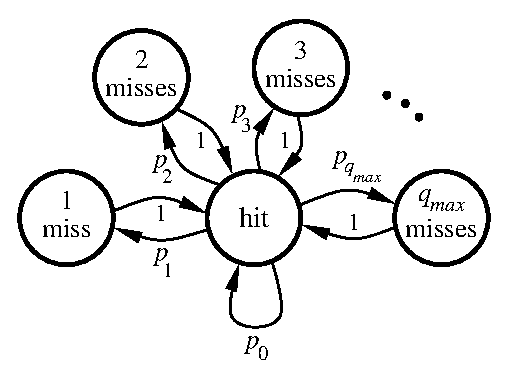
\includegraphics[scale=0.7]{\figdir/misses.eps}}
    \caption{Markov model for the random sequence of hits and misses.}
    \label{fig:Markov}
\end{figure}

We model the task execution as a random process, assuming that the pattern of hits and misses in the real-time system is described by the homogeneous Markov model shown in Figure~\ref{fig:Markov}.
In this model, after each hit, the system will experience a miss interval of length $\counter \in \{0,\ldots,\counter_\mathit{max}\}$ with independent probability $p_\counter$. Naturally, $\sum_{i=0}^{\counter_\mathit{max}} p_i = 1$.

In each interval, the system will experience $\counter$ deadline misses followed by one deadline hit. Iterating \eqref{eq:covariance} over said interval, the covariance will then develop as
\begin{equation*}
    \label{eq:intervalP}
    \begin{aligned}
    \Pi_{k+q+1} &= \Phi_\mathit{hit}(\counter)  \Bigl((\Phi_\mathit{miss})^\counter \Pi_k (\Phi_\mathit{miss}^{\T})^\counter \Bigr.\\
    &\Bigl.+ \textstyle\sum_{i=0}^{q-1} (\Phi_\mathit{miss})^i \Gamma R \Gamma^{\T} (\Phi_\mathit{miss}^{\T})^i \Bigr)\Phi_\mathit{hit}^{\T}(\counter)  \\
    &+ \Gamma R \Gamma^{\T} .
    \end{aligned}
\end{equation*}
The time-varying closed-loop system together with the Markov model define a \emph{discrete-time Markov jump linear system} for which well-established results exist (e.g., \cite{Blair:1975,Nilsson:1998,Lincoln:2002}). Using this theory, it is possible to calculate the \emph{stationary} (time-averaged) state covariance, denoted $\overline\Pi$. With this, the performance \eqref{eq:cost} can finally be obtained as
\begin{equation*}
    J = \operatorname{trace} \funof{ \overline\Pi \, \overline{Q} },
\end{equation*}
where
\begin{equation*}
    \overline{Q} = \begin{bmatrix}
    C^{\T}Q C & 0 \\ 0 & 0_{n_z+n_y+n_u}
    \end{bmatrix}.
\end{equation*}

% From here, given the likelihood $p_\counter$ of each miss interval length $\counter$, the \emph{stationary} state variance $\Pi = \underset{q}{\mathbb{E}} \left[ \xi_k \cdot \xi_k^{\T} \right]$ after a hit satisfies
% \begin{equation}
%     \label{eq:expected-pi}
%     \Pi  =\underset{q}{\mathbb{E}} \left[ \Pi_{k+q+1} \right] =
%     \sum_{q=0}^{q_\mathit{max}} p_q \Pi_{k+q+1}.
% \end{equation}
% %
% By imposing the convergence of $\Pi=\Pi_{k+q+1}=\Pi_{k}$, and substituting Equation~\eqref{eq:intervalP} in Equation~\eqref{eq:expected-pi}, we obtain
% %
% \begin{equation}
%     \begin{aligned}
%     \Pi &= \sum_{q=0}^{q_\mathit{max}} p_q \Bigl[ \Phi_\mathit{hit}(\counter)  (\Phi_\mathit{miss})^\counter \Pi (\Phi_\mathit{miss}^{\T})^\counter  \Phi_\mathit{hit}(q)^{\T} \Bigr.\\
%     &+ \sum_{i=0}^{q-1}  \Phi_\mathit{hit}(\counter) (\Phi_\mathit{miss})^i \Gamma R_w \Gamma^{\T} (\Phi_\mathit{miss}^{\T})^i \Phi_\mathit{hit}^{\T}(\counter)  \Bigl. \Bigr] \\
%     &+ \Gamma R_w \Gamma^{\T} .
%     \end{aligned}
% \end{equation}
% This linear matrix equation can be solved analytically or by iteration. Once $\Pi$ has been found, the expected covariance during the miss intervals can be calculated from \eqref{eq:covariance}. \nv{Up until here I think it clear now!}
% Finally, the time-average performance is given by
% \revise{
% \begin{equation}
%     J = \E{ y_k^{\T} Q y_k } =  \operatorname{trace}\funof{\Pi_k \begin{bmatrix}
% C^{\T} Q C & 0 \\ 0 & 0_{n_z+n_y+n_w} \end{bmatrix}}.
%     \label{eq:J}
% \end{equation}
% }

% To compare the performance of two closed-loop systems $a$ and $b$, we evaluate the weighted mean-square difference between their outputs:

To compare the performance of different implementations, we first define the \emph{ideal performance} as the cost $J$ obtained when there are no deadline misses (i.e., $p_0 = 1$ and $p_i = 0$, $i \geq 1$).
We then obtain the \emph{relative performance degradation} of an arbitrary controller $\ctrler^{\dagger}$ by calculating the weighted mean-square difference between the actual and ideal systems' outputs, $y^{\dagger}_k$ and $y_k$ respectively, and normalising it with respect to the ideal performance $J$:
\begin{equation}
    \label{eq:relcost}
%   \Delta J = \E{ (y^a_k - y^b_k)^{\T} Q (y^a_k - y^b_k) }.
  \frac{\Delta J^{\dagger}}{J} = \frac{\E{ (y^{\dagger}_k - y_k)^{\T} Q (y^{\dagger}_k - y_k) }}{ \E{ y_k^{\T} Q y_k }}.
\end{equation}
This can be found by analysing both systems in parallel when driven by the same noise sequence $w_k$:
\begin{equation*}
    \begin{bmatrix}
    \xi_{k+1}^\dagger \\ \xi_{k+1}%^b 
    \end{bmatrix} =
    \begin{bmatrix}
    \Phi_k^\dagger & 0 \\ 0 & \Phi_k%^b
    \end{bmatrix}
    \begin{bmatrix}
    \xi_k^\dagger \\ \xi_k%^b 
    \end{bmatrix} +
    \begin{bmatrix}
    \Gamma \\ \Gamma
    \end{bmatrix} w_k
\end{equation*}
After finding the stationary state covariance $\overline{\Pi}_e$ of this extended system (using the same technique as referred to above), we can retrieve the absolute performance difference as
\begin{equation*}
    \label{eq:deltaJ}
 \Delta J^{\dagger} = \operatorname{trace} \funof{ \overline{\Pi}_e  \begin{bmatrix}
    \phantom{-}\overline{Q} & -\overline{Q}\phantom{,} \\
    -\overline{Q} & \phantom{-}\overline{Q}\phantom{,}
    \end{bmatrix} }.
\end{equation*}

%The performance difference is finally obtained as
%\begin{equation}
%    \Delta J = \E{ \begin{bmatrix}
%    \xi_k^\dagger \\ \xi_k%^b 
%    \end{bmatrix}^{\T}
%    \begin{bmatrix}
%    C^{\T}QC & 0 & -C^{\T}QC & 0 \\
%    0 & 0 & 0 & 0 \\
%    -C^{\T}QC & 0 & C^{\T}QC & 0 \\
%    0 & 0 & 0 &  0
%    \end{bmatrix}
%    \begin{bmatrix}
%    \xi_k^\dagger \\ \xi_k%^b 
%    \end{bmatrix}
%    } .
%\end{equation}


\section{Experimental Evaluation}
\label{sec:results}
In this section, we apply the analysis presented in Section~\ref{sec:analysis} to a set of case studies, analysing stability and performance. 
We first present detailed results with a Furuta pendulum, both in simulation and with real hardware, using the same controller. 
The simulated results are compared to the real physical plant. 
This shows that the performance analysis does capture the important trends for real control systems.
We then present some aggregate results obtained with a set of 133 different plants from a control benchmark.
One noteworthy aspect is that the Furuta pendulum model is linearised for the control design and the pendulum stabilised around an unstable equilibrium---the top position---while the control benchmark includes (by design) stable systems. 
The difference between simulation results and real experiments for stable linear systems should in principle be smaller than for unstable nonlinear systems, making our pendulum the ideal stress test for the similarity of simulated and real data.

\subsection{Furuta Pendulum}
\label{sec:example}

We here analyse the behaviour of a Furuta pendulum~\cite{Furuta:1992}, a rotational inverted pendulum in which a rotating arm is connected to a pendulum. 
The rotation of the arm induces a swing movement on the pendulum. 
The pendulum has two equilibria: a stable position in which the pendulum is downright, and an unstable position in which the pendulum is upright. 
Our objective is to keep the pendulum in the up position, by moving the rotating arm.

The Furuta pendulum is a highly nonlinear process. 
In order to design a control strategy to keep the pendulum in the top position, it is necessary to linearise the dynamics of the system around the desired equilibrium point. 
We consider this as a stress test to check the divergence between simulation results and real hardware results, because of the instability of the equilibrium and the nonlinearity of the dynamics. 
In fact, the controller necessarily acts with information that is valid only around the upright position, and there is only a range of states in which the linearised model closely describes the behaviour of the physical plant.

We design a linear-quadratic regulator (LQR) to control the plant. 
Every $\Ts=10\,$ms the plant is sampled and the control signal is actuated.
Based on state-of-the-art models~\cite{Cazzolato:2011} and on our control design, the plant model $\plant$ is
\begin{equation}
    \label{eq:furuta}
    \setlength\arraycolsep{2pt}
    \begin{aligned}
        \plant \,\, : \,\, & \left\{ 
        \begin{aligned}
            x_{t+1} &= 
            \begin{bmatrix*}[c] 
                1.002 & 0.0100 & 0 & 0 \\
                0.3133 & 1.002 & 0 & 0 \\
                -2.943\cdot 10^{-5} & -9.808\cdot 10^{-8} & 1 & 0.01 \\
                -0.0059 & -2.943\cdot 10^{-5} & 0 & 1
            \end{bmatrix*} x_t + 
            \begin{bmatrix*}[c]
                -0.0036 \\
                -0.7127 \\
                \textcolor{white}{+}0.0096 \\
                \textcolor{white}{+}1.9120
            \end{bmatrix*} u_t + I w_t,\\
            y_t &= I x_t, 
        \end{aligned} \right. \\
    \end{aligned}
\end{equation}
the controller $\ctrler$ takes the form
\begin{equation}
    \label{eq:furuta2}
    \begin{aligned}
        \ctrler \,\, : \,\,\, & u_{t+1} = 
        \begin{bmatrix*}[c]
        8.8349 & 1.5804 & 0.2205 & 0.3049
        \end{bmatrix*} x_t 
    \end{aligned}
\end{equation}
and is designed and analysed using the following parameters (see Section~\ref{sec:cldynamics}):
\begin{equation}
    \label{eq:furuta3}
    \begin{aligned}
        Q_e &= \diag{100,1,10,10}, \,\,\, Q_u = 100, \,\,\, R = \diag{0, 0, 10, 1}.
    \end{aligned}
\end{equation}

We first apply the stability analyses presented in Section~\ref{sec:derivation} to our model.
\begin{figure}[t]
    \centerline{\resizebox{0.95\textwidth}{!}{\pgfplotstableread[header=false,col sep=comma]{\figdir/data/stability-furuta/KH-stability.csv}\kh%
\pgfplotstableread[header=false,col sep=comma]{\figdir/data/stability-furuta/KZ-stability.csv}\kz%
\pgfplotstableread[header=false,col sep=comma]{\figdir/data/stability-furuta/SH-stability.csv}\sh%
\pgfplotstableread[header=false,col sep=comma]{\figdir/data/stability-furuta/SZ-stability.csv}\sz%

% they all have the same number of columns and rows
\pgfplotstablegetrowsof{\kh}
\pgfmathtruncatemacro{\numrows}{\pgfplotsretval}
\pgfplotstablegetcolsof{\kh}
\pgfmathtruncatemacro{\numcols}{\pgfplotsretval}

\centering

\begin{tikzpicture}[scale=0.096]
    \small

    \draw[thick] (0,0) -- (0,50) -- (25,50) -- (25,0) -- cycle;
    \draw[dashed] (-1,0.5) node[left] {$1$} -- (0,0.5);
    \draw[dashed] (-1,9.5) node[left] {$10$} -- (0,9.5);
    \draw[dashed] (-1,19.5) node[left] {$20$} -- (0,19.5);
    \draw[dashed] (-1,29.5) node[left] {$30$} -- (0,29.5);
    \draw[dashed] (-1,39.5) node[left] {$40$} -- (0,39.5);
    \draw[dashed] (-1,49.5) node[left] {$50$} -- (0,49.5);

    \draw[dashed] (0.5,-1) node[below] {$1$} -- (0.5,0);
    \draw[dashed] (4.5,-1) node[below] {$5$} -- (4.5,0);
    \draw[dashed] (9.5,-1) node[below] {$10$} -- (9.5,0);
    \draw[dashed] (14.5,-1) node[below] {$15$} -- (14.5,0);
    \draw[dashed] (19.5,-1) node[below] {$20$} -- (19.5,0);
    \draw[dashed] (24.5,-1) node[below] {$25$} -- (24.5,0);

    \foreach \Y [evaluate=\Y as \PrevY using {int(\numrows-\Y)},
    evaluate=\Y as \NewY using {int(\numrows-\Y+1)}] in {1,...,\numrows}{
        \foreach \X  [evaluate=\X as \PrevX using {int(\X-1)}] in {1,...,\numcols}{
            \ReadOutElement{\kh}{\PrevY}{\PrevX}{\Current}
            % our class
            \ifnum\Current=0 \def\colorcell{white} \fi
            \ifnum\Current=2 \def\colorcell{blue!30} \fi
            \ifnum\Current=3 \def\colorcell{blue} \fi

            \draw[black,densely dotted,fill=\colorcell] (\PrevX,\numrows-\PrevY-1) rectangle +(1,1);
        }
        }
        % title and axis
        \node at (12.5,52.5) {\textbf{Kill\&Hold}};
        %\node[rotate=90] at (-7.5,25) {$m$};
        \node[] at (12.5,-6.5) {$n$};
        \node[rotate=90] at (-7.5,25) {$m$};
\end{tikzpicture}
\hspace{-1mm}
\begin{tikzpicture}[scale=0.096]
    \small

    \draw[thick] (0,0) -- (0,50) -- (25,50) -- (25,0) -- cycle;
    \draw[dashed] (-1,0.5) node[left] {$1$} -- (0,0.5);
    \draw[dashed] (-1,9.5) node[left] {$10$} -- (0,9.5);
    \draw[dashed] (-1,19.5) node[left] {$20$} -- (0,19.5);
    \draw[dashed] (-1,29.5) node[left] {$30$} -- (0,29.5);
    \draw[dashed] (-1,39.5) node[left] {$40$} -- (0,39.5);
    \draw[dashed] (-1,49.5) node[left] {$50$} -- (0,49.5);

    \draw[dashed] (0.5,-1) node[below] {$1$} -- (0.5,0);
    \draw[dashed] (4.5,-1) node[below] {$5$} -- (4.5,0);
    \draw[dashed] (9.5,-1) node[below] {$10$} -- (9.5,0);
    \draw[dashed] (14.5,-1) node[below] {$15$} -- (14.5,0);
    \draw[dashed] (19.5,-1) node[below] {$20$} -- (19.5,0);
    \draw[dashed] (24.5,-1) node[below] {$25$} -- (24.5,0);

    \foreach \Y [evaluate=\Y as \PrevY using {int(\numrows-\Y)},
    evaluate=\Y as \NewY using {int(\numrows-\Y+1)}] in {1,...,\numrows}{
        \foreach \X  [evaluate=\X as \PrevX using {int(\X-1)}] in {1,...,\numcols}{
            \ReadOutElement{\sh}{\PrevY}{\PrevX}{\Current}
            % our class
            \ifnum\Current=0 \def\colorcell{white} \fi
            \ifnum\Current=2 \def\colorcell{pink} \fi
            \ifnum\Current=3 \def\colorcell{pink!75!black} \fi

            \draw[black,densely dotted,fill=\colorcell] (\PrevX,\numrows-\PrevY-1) rectangle +(1,1);
        }
        }
        % title and axis
        \node at (12.5,52.5) {\textbf{Skip\&Hold}};
        %\node[rotate=90] at (-7.5,25) {$m$};
        \node[] at (12.5,-6.5) {$n$};
\end{tikzpicture}
\hspace{-1mm}
\begin{tikzpicture}[scale=0.096]
    \small

    \draw[thick] (0,0) -- (0,50) -- (25,50) -- (25,0) -- cycle;
    \draw[dashed] (-1,0.5) node[left] {$1$} -- (0,0.5);
    \draw[dashed] (-1,9.5) node[left] {$10$} -- (0,9.5);
    \draw[dashed] (-1,19.5) node[left] {$20$} -- (0,19.5);
    \draw[dashed] (-1,29.5) node[left] {$30$} -- (0,29.5);
    \draw[dashed] (-1,39.5) node[left] {$40$} -- (0,39.5);
    \draw[dashed] (-1,49.5) node[left] {$50$} -- (0,49.5);

    \draw[dashed] (0.5,-1) node[below] {$1$} -- (0.5,0);
    \draw[dashed] (4.5,-1) node[below] {$5$} -- (4.5,0);
    \draw[dashed] (9.5,-1) node[below] {$10$} -- (9.5,0);
    \draw[dashed] (14.5,-1) node[below] {$15$} -- (14.5,0);
    \draw[dashed] (19.5,-1) node[below] {$20$} -- (19.5,0);
    \draw[dashed] (24.5,-1) node[below] {$25$} -- (24.5,0);

    \foreach \Y [evaluate=\Y as \PrevY using {int(\numrows-\Y)},
    evaluate=\Y as \NewY using {int(\numrows-\Y+1)}] in {1,...,\numrows}{
        \foreach \X  [evaluate=\X as \PrevX using {int(\X-1)}] in {1,...,\numcols}{
            \ReadOutElement{\kz}{\PrevY}{\PrevX}{\Current}
            % our class
            \ifnum\Current=0 \def\colorcell{white} \fi
            \ifnum\Current=2 \def\colorcell{cyan!30} \fi
            \ifnum\Current=3 \def\colorcell{cyan} \fi

            \draw[black,densely dotted,fill=\colorcell] (\PrevX,\numrows-\PrevY-1) rectangle +(1,1);
        }
        }
        % title and axis
        \node at (12.5,52.5) {\textbf{Kill\&Zero}};
        \node[] at (12.5,-6.5) {$n$};
\end{tikzpicture}
\hspace{-1mm}
\begin{tikzpicture}[scale=0.096]
    \small

    \draw[thick] (0,0) -- (0,50) -- (25,50) -- (25,0) -- cycle;
    \draw[dashed] (-1,0.5) node[left] {$1$} -- (0,0.5);
    \draw[dashed] (-1,9.5) node[left] {$10$} -- (0,9.5);
    \draw[dashed] (-1,19.5) node[left] {$20$} -- (0,19.5);
    \draw[dashed] (-1,29.5) node[left] {$30$} -- (0,29.5);
    \draw[dashed] (-1,39.5) node[left] {$40$} -- (0,39.5);
    \draw[dashed] (-1,49.5) node[left] {$50$} -- (0,49.5);

    \draw[dashed] (0.5,-1) node[below] {$1$} -- (0.5,0);
    \draw[dashed] (4.5,-1) node[below] {$5$} -- (4.5,0);
    \draw[dashed] (9.5,-1) node[below] {$10$} -- (9.5,0);
    \draw[dashed] (14.5,-1) node[below] {$15$} -- (14.5,0);
    \draw[dashed] (19.5,-1) node[below] {$20$} -- (19.5,0);
    \draw[dashed] (24.5,-1) node[below] {$25$} -- (24.5,0);

    \foreach \Y [evaluate=\Y as \PrevY using {int(\numrows-\Y)},
    evaluate=\Y as \NewY using {int(\numrows-\Y+1)}] in {1,...,\numrows}{
        \foreach \X  [evaluate=\X as \PrevX using {int(\X-1)}] in {1,...,\numcols}{
            \ReadOutElement{\sz}{\PrevY}{\PrevX}{\Current}
            % our class
            \ifnum\Current=0 \def\colorcell{white} \fi
            \ifnum\Current=2 \def\colorcell{red!30} \fi
            \ifnum\Current=3 \def\colorcell{red} \fi

            \draw[black,densely dotted,fill=\colorcell] (\PrevX,\numrows-\PrevY-1) rectangle +(1,1);
        }
        }
        % title and axis
        \node at (12.5,52.5) {\textbf{Skip\&Zero}};
        %\node[rotate=90] at (-7.5,25) {$m$};
        \node[] at (12.5,-6.5) {$n$};
\end{tikzpicture}
}}
    \caption{Miss-constrained stability (dark coloured area) and \nilsstability{} stability (light coloured area) when different strategies $\strat$ are used in the example and the weakly hard model in Definition~\ref{def:task-model} is considered.
        Each square represents a window of size $\ell = \nummisses+\numhits$.
        The dark area satisfies both the \switchingstability{} and \nilsstability{} stability whilst the light area only provides \nilsstability{} stability.
        The white squares denote potentially unstable combinations of $\nummisses$ and $\numhits$.}
    \label{fig:stability_extended}
\end{figure}
Figure~\ref{fig:stability_extended} shows the results. Each square in the figure represents a combination of (at most) $m$ deadline misses (on the vertical axis) and (at least) $n$ deadline hits (on the horizontal axis).
If a square is coloured with a dark colour, the corresponding combination of misses and hits is both \nilsstability{} and \switchingstability{} stable, found using the \code{JSR Toolbox}~\cite{Jungers:2014}. 
The light squares in the figure show combinations for which the system only satisfies the \nilsstability{} stability condition. 
The white squares mark configurations for which stability cannot be guaranteed.

We remark on the presence of peaks in the \nilsstability{} stability region of $\strat = KH$ at $\numhits = \{1, 5, 9, 13, 19\}$.
Similar peaks are also found for the other strategies, but for different values of $\numhits$.
These peaks indicate that the system would be stable if that particular burst and recovery interval length would be repeated indefinitely.
However, this assumption is not robust to variations in the burst or recovery interval lengths as can be seen from the \switchingstability{} stability region being more conservative with its guarantees.
Instead, the peaks in the \nilsstability{} region can be explained by stable modes occurring due to the natural frequencies of the open-loop (for the \tZ{} actuation mode) and closed-loop (for the \tH{} actuation mode) systems.
It is also interesting to note that \tK{} seems to consistently yield a larger stability region than \tS{}, while neither \tZ{} nor \tH{} dominate each other in terms of stability guarantees. An example of the latter fact was given already in~\cite{schenato09}.

For the performance analysis, we considered a one-shot burst fault of a specific length $m$, followed by a long period of normal execution. 
Assuming that the pendulum starts close to the upright equilibrium, with stationary cost $J_\infty$, we calculate how the covariance $P_t$ and performance cost $J_t$ evolve during and after the burst interval using Equations~\eqref{eq:covariance-evolution}--\eqref{eq:evolutionparameters}.\footnote{The analysis is implemented using \code{JitterTime}~\cite{Cervin:2019}, \url{https://www.control.lth.se/jittertime}.} 
These calculations assume an ideal, linear model of the pendulum. 
The simulation results for different strategies and bursts of length $m=20$ are shown in the upper half of Figure~\ref{fig:cost_simvsreal}. 
For \tH{}, it is seen that the cost grows exponentially during the initial fault interval (the first $20\,\Ts=0.2\,$s). 
This is true also for \tZ{}, although the growth rate is too small to be visible.
The reason for the poor performance of \tH{} is that any non-zero held control signal will actively push the pendulum away from its unstable upright equilibrium even further than either disturbances or noise would already do without a proper control action.
%
\begin{figure}
    \centering
    \begin{tikzpicture}
\small

\def \fkhj {\figdir/data/experiment-JT-data/KH.csv}
\def \fkzj {\figdir/data/experiment-JT-data/KZ.csv}
\def \fshj {\figdir/data/experiment-JT-data/SH.csv}
\def \fszj {\figdir/data/experiment-JT-data/SZ.csv}
\def \fkhr {\figdir/data/experiment-data/kill-hold-20-480.csv}
\def \fkzr {\figdir/data/experiment-data/kill-zero-20-480.csv}
\def \fshr {\figdir/data/experiment-data/skip-hold-20-480.csv}
\def \fszr {\figdir/data/experiment-data/skip-zero-20-480.csv}

\begin{groupplot}[%clip mode=individual,
     group style = {group size = 4 by 2, horizontal sep = 7mm, vertical sep=5mm},
     height = 0.3\textwidth,
     width = 0.3\textwidth,
     enlargelimits=false,
     ymin=0,
     grid = both,
     grid style = {dashed, black!20},
     xlabel near ticks,
     ylabel near ticks,
     cyan,
     ultra thick,
     mark=none,
     mark options={fill=white}]

    \nextgroupplot[ylabel = \textbf{$J_k/J_\infty$ Simulated}, ymax=57, ymin=-5, ytick={1,10,30,50}]
    \node[clip=false, anchor=south] at (axis cs:1,57) {\textbf{\textcolor{white}{p}Kill\&Hold\textcolor{white}{p}}};
    \pgfplotstableread[header=true,col sep=comma]{\fkhj}\extdata;
    \addplot[mark max, blue] table[x expr=\thisrow{T}*0.01, y=J, col sep=comma] {\extdata};

    \nextgroupplot[ymax=57, ymin=-5,ytick={1,10,30,50}]
    \node[clip=false, anchor=south] at (axis cs:1,57) {\textbf{Skip\&Hold}};
    \pgfplotstableread[header=true,col sep=comma]{\fshj}\extdata;
    \addplot[mark max, pink!75!black] table[x expr=\thisrow{T}*0.01, y=J, col sep=comma] {\extdata};

    \nextgroupplot[ymax=10, ytick={1,3,5,7}]
    \node[clip=false, anchor=south] at (axis cs:1,10) {\textbf{\textcolor{white}{p}Kill\&Zero\textcolor{white}{p}}};
    \pgfplotstableread[header=true,col sep=comma]{\fkzj}\extdata;
    \addplot[mark max, cyan] table[x expr=\thisrow{T}*0.01, y=J, col sep=comma] {\extdata};

    \nextgroupplot[ymax=10, ytick={1,3,5,7}]
    \node[clip=false, anchor=south] at (axis cs:1,10) {\textbf{Skip\&Zero}};
    \pgfplotstableread[header=true,col sep=comma]{\fszj}\extdata;
    \addplot[mark max, red] table[x expr=\thisrow{T}*0.01, y=J, col sep=comma] {\extdata};
      
    \nextgroupplot[xlabel = {Time [s]}, ylabel = \textbf{$J_k/J_\infty$ Real}, ymax=57, ymin=-5, ytick={1,10,30,50}]
    \pgfplotstableread[header=true,col sep=comma]{\fkhr}\extdata;
    \addplot[mark max, blue] table[x expr=\thisrow{T}*0.01, y=J, col sep=comma] {\extdata};

    \nextgroupplot[xlabel = {Time [s]}, ymax=57, ymin=-5,ytick={1,10,30,50}]
    \pgfplotstableread[header=true,col sep=comma]{\fshr}\extdata;
    \addplot[mark max, pink!75!black] table[x expr=\thisrow{T}*0.01, y=J, col sep=comma] {\extdata};

    \nextgroupplot[xlabel = {Time [s]}, ymax=10, ytick={1,3,5,7}]
    \pgfplotstableread[header=true, col sep=comma]{\fkzr}\extdata;
    \addplot[mark max, cyan] table[x expr=\thisrow{T}*0.01, y=J, col sep=comma] {\extdata};

    \nextgroupplot[xlabel = {Time [s]}, ymax=10, ytick={1,3,5,7}]
    \pgfplotstableread[header=true,col sep=comma]{\fszr}\extdata;
    \addplot[mark max, red] table[x expr=\thisrow{T}*0.01, y=J, col sep=comma] {\extdata};

\end{groupplot}
\end{tikzpicture}

    \caption{Normalised performance cost $J_t/J_\infty$ obtained with the Furuta pendulum.
        The upper part of the figure shows simulated data, while the lower part of the figure shows the corresponding values obtained averaging the results of 500 experiments with the real process and hardware.
        Each experiment corresponds to a 500 jobs of the controller (20 misses and 480 hits).}
    \label{fig:cost_simvsreal}
\end{figure}


The large spike in cost comes when the controller is reactivated at time $0.2\,$s. 
Here, the \tH{} strategy again shows much worse performance than \tZ{}, with the peak cost being almost an order of magnitude worse. 
The difference between \tK{} and \tS{} is relatively small, with the latter strategy consistently performing slightly worse than the former. 
This is due to the small extra delay caused by using old data in the \tS{} strategy.

We conducted experiments on a Furuta pendulum, using the same controller for the real plant rather than its model.\footnote{A video, showing experiments with the real system and bursts of deadline misses can be viewed at \url{https://youtu.be/0P0K_7lvKVU}. The video shows a comparison of all the strategies for bursts of $(m = 20, n=480)$. Furthermore, we have included additional experiments with $(m=50, n=450)$ and $(m=75, n=425)$ for the \tSH{} strategy. The results of the additional experiments with higher values of $m$ are not described in the paper, as stability could not be guaranteed (and in fact the pendulum is not at all times kept in the upright position).}
Initially, we performed 500 experiments with 500 jobs each and no deadline misses, to determine the nominal variance of the system---i.e., the stationary variance used to find the static cost $J_\infty$.
For each strategy $\strat$ we then ran 500 identically set up experiments. 
In each experiment, the control task operated according to the task model from Definition~\ref{def:task-model}, experiencing a burst of length $\nummisses=20$ misses, followed by by a recovery interval with $\numhits=480$ deadline hits.

Due to system model uncertainties (e.g., friction) being significant, the rotation angle around the arm axis displayed a considerable variance.
We removed the state from the covariance calculations, since the arm angle majorly impacted the variance despite its inconsequential significance on the system dynamics (the pendulum can be stabilised with the arm being around any position, provided that the pendulum itself is kept in the upright position).
Including the rotation angle would not change the shape of the performance degradation seen in Figure~\ref{fig:cost_simvsreal}. 
However, it would make the results obtained with different strategies $\strat$ not comparable (in some of them, the rotation angle could have varied less across the 500 experiments). 
The covariance matrix $P_t$ was derived by calculating the variance of the closed-loop state vector $\tilde{x}_t$ according to Equation~\eqref{eq:covarcalc}, in each time step $t$. 

The resulting performance cost can be seen in the lower half of Figure~\ref{fig:cost_simvsreal}, where the cost $J_t$ was calculated according to Equation~\eqref{eq:covartocost} and normalised using the stationary cost $J_\infty$. 
Comparing the simulated (upper) and real (lower) performance costs in Figure~\ref{fig:cost_simvsreal}, we notice the similarities between the simulated analysis and the analysis performed on the physical plant. 
%
Particularly, the strategies involving \tH{} actuation show similar behaviours. 
For these strategies, the simulated and real values are very close for the transient burst interval, the secondary cost peak (seen around time $0.4\,$s), and the maximum normalised cost $J_{M, \strat}$.
However, the real cost is recovering slower than in the simulations---an effect that arises due to the nonlinear effects present in the real process, but unmodelled in the simulated environment.
%
Instead, comparing the \tZ{} actuation strategies, the performance cost of the physical experiments during the burst interval seem to improve compared to the simulations.
This is again likely due to the unmodelled dynamics (e.g., friction) appearing in the physical experiment but not in the simulations.
The stiction component of the friction reduces the variance of the states when the actuation signal becomes zero.
With longer burst intervals, a similar behaviour as for the \tH{} actuation strategies would appear.
Despite this difference, both the recovery interval, the secondary cost peak (around $0.4\,$s), and the maximum normalised costs $J_{M,\strat}$ are comparable.

We conclude that the results of the experiments performed on the physical process support the validity of the performance analysis presented in Section~\ref{sec:derivation}.

\subsection{Control Benchmark}
\label{sec:aggregateresults}

In Section~\ref{sec:example} we extensively discussed the results obtained with a single plant (the Furuta pendulum), with the aim of showing that simulating the performance cost yields interesting and relevant results.
As the main novelty of this paper lays in the introduction of the performance analysis as an additional tool to evaluate the behaviour of control systems that can miss deadlines, we here focus on performance.

\begin{figure}[t]
    \centering
    \resizebox{0.95\textwidth}{!}{\begin{tikzpicture}[bar width=1mm]
\small

\begin{groupplot}[group style = {group size = 4 by 9, vertical sep=8mm, horizontal sep=8mm},
    height = 3.05cm,
    width = 4cm,
    ybar,
    ymin = 0,
    ylabel style={at={(-0.35,1)}, anchor=east},
    grid = major,
    grid style = {dashed, black!20},
    x tick label style = {rotate = 60, anchor=north east, inner sep = 0mm},
    xtick distance=1, enlarge x limits=0.05,
    extra x ticks={1}]

    \nextgroupplot[title={\textbf{\textcolor{white}{p}Kill\&Hold\textcolor{white}{p}}}, ymax=70, ylabel={\textbf{$\,\,$Batch 1}},
    xtick distance=3, enlarge x limits=0.02]
    \addplot[thin, black, fill=blue] table[x=ID, y=HITS, col sep=comma]
    {\figdir/data/processed/B1_KH_10.csv};

    \nextgroupplot[title={\textbf{Skip\&Hold}}, ymax=70,
    xtick distance=3, enlarge x limits=0.02]
    \addplot[thin, black, fill=pink!75!black] table[x=ID, y=HITS, col sep=comma]
    {\figdir/data/processed/B1_SH_10.csv};

    \nextgroupplot[title={\textbf{\textcolor{white}{p}Kill\&Zero\textcolor{white}{p}}}, ymax=70,
    xtick distance=3, enlarge x limits=0.02]
    \addplot[thin, black, fill=cyan] table[x=ID, y=HITS, col sep=comma]
    {\figdir/data/processed/B1_KZ_10.csv};

    \nextgroupplot[title={\textbf{Skip\&Zero}}, ymax=70,
    xtick distance=3, enlarge x limits=0.02]
    \addplot[thin, black, fill=red] table[x=ID, y=HITS, col sep=comma]
    {\figdir/data/processed/B1_SZ_10.csv};

    % ------------------------------------------------------

    \nextgroupplot[ymax=120, ylabel={\textbf{$\,\,$Batch 2}},
    xtick distance=3, enlarge x limits=0.02]
    \addplot[thin, black, fill=blue] table[x=ID, y=HITS, col sep=comma]
    {\figdir/data/processed/B2_KH_10.csv};

    \nextgroupplot[ymax=120,
    xtick distance=3, enlarge x limits=0.02]
    \addplot[thin, black, fill=pink!75!black] table[x=ID, y=HITS, col sep=comma]
    {\figdir/data/processed/B2_SH_10.csv};

    \nextgroupplot[ymax=120,
    xtick distance=3, enlarge x limits=0.02]
    \addplot[thin, black, fill=cyan] table[x=ID, y=HITS, col sep=comma]
    {\figdir/data/processed/B2_KZ_10.csv};

    \nextgroupplot[ymax=120,
    xtick distance=3, enlarge x limits=0.02]
    \addplot[thin, black, fill=red] table[x=ID, y=HITS, col sep=comma]
    {\figdir/data/processed/B2_SZ_10.csv};

    % ------------------------------------------------------

    \nextgroupplot[ymax=90, ylabel={\textbf{$\,\,$Batch 3}}]
    \addplot[thin, black, fill=blue] table[x=ID, y=HITS, col sep=comma]
    {\figdir/data/processed/B3_KH_10.csv};

    \nextgroupplot[ymax=90]
    \addplot[thin, black, fill=pink!75!black] table[x=ID, y=HITS, col sep=comma]
    {\figdir/data/processed/B3_SH_10.csv};

    \nextgroupplot[ymax=90]
    \addplot[thin, black, fill=cyan] table[x=ID, y=HITS, col sep=comma]
    {\figdir/data/processed/B3_KZ_10.csv};

    \nextgroupplot[ymax=90]
    \addplot[thin, black, fill=red] table[x=ID, y=HITS, col sep=comma]
    {\figdir/data/processed/B3_SZ_10.csv};

    % ------------------------------------------------------

    \nextgroupplot[ymax=70,
    ylabel={\textbf{$\,\,$Batch 4}}]
    \addplot[thin, black, fill=blue] table[x=ID, y=HITS, col sep=comma]
    {\figdir/data/processed/B4_KH_10.csv};

    \nextgroupplot[ymax=70]
    \addplot[thin, black, fill=pink!75!black] table[x=ID, y=HITS, col sep=comma]
    {\figdir/data/processed/B4_SH_10.csv};

    \nextgroupplot[ymax=70]
    \addplot[thin, black, fill=cyan] table[x=ID, y=HITS, col sep=comma]
    {\figdir/data/processed/B4_KZ_10.csv};

    \nextgroupplot[ymax=70]
    \addplot[thin, black, fill=red] table[x=ID, y=HITS, col sep=comma]
    {\figdir/data/processed/B4_SZ_10.csv};

    % ------------------------------------------------------

    \nextgroupplot[ymax=100,
    ylabel={\textbf{$\,\,$Batch 5}}]
    \addplot[thin, black, fill=blue] table[x=ID, y=HITS, col sep=comma]
    {\figdir/data/processed/B5_KH_10.csv};

    \nextgroupplot[ymax=100]
    \addplot[thin, black, fill=pink!75!black] table[x=ID, y=HITS, col sep=comma]
    {\figdir/data/processed/B5_SH_10.csv};

    \nextgroupplot[ymax=100]
    \addplot[thin, black, fill=cyan] table[x=ID, y=HITS, col sep=comma]
    {\figdir/data/processed/B5_KZ_10.csv};

    \nextgroupplot[ymax=100]
    \addplot[thin, black, fill=red] table[x=ID, y=HITS, col sep=comma]
    {\figdir/data/processed/B5_SZ_10.csv};

    % ------------------------------------------------------

    \nextgroupplot[ymax=120,
    ylabel={\textbf{$\,\,$Batch 6}}]
    \addplot[thin, black, fill=blue] table[x=ID, y=HITS, col sep=comma]
    {\figdir/data/processed/B6_KH_10.csv};

    \nextgroupplot[ymax=120]
    \addplot[thin, black, fill=pink!75!black] table[x=ID, y=HITS, col sep=comma]
    {\figdir/data/processed/B6_SH_10.csv};

    \nextgroupplot[ymax=120]
    \addplot[thin, black, fill=cyan] table[x=ID, y=HITS, col sep=comma]
    {\figdir/data/processed/B6_KZ_10.csv};

    \nextgroupplot[ymax=120]
    \addplot[thin, black, fill=red] table[x=ID, y=HITS, col sep=comma]
    {\figdir/data/processed/B6_SZ_10.csv};


    % ------------------------------------------------------

    \nextgroupplot[ymax=120, ylabel={\textbf{$\,\,$Batch 7}},
    xtick distance=5, enlarge x limits=0.02]
    \addplot[thin, black, fill=blue, bar width=0.6mm] table[x=ID, y=HITS, col sep=comma]
    {\figdir/data/processed/B7_KH_10.csv};

    \nextgroupplot[ymax=120,
    xtick distance=5, enlarge x limits=0.02]
    \addplot[thin, black, fill=pink!75!black, bar width=0.6mm] table[x=ID, y=HITS, col sep=comma]
    {\figdir/data/processed/B7_SH_10.csv};

    \nextgroupplot[ymax=120,
    xtick distance=5, enlarge x limits=0.02]
    \addplot[thin, black, fill=cyan, bar width=0.6mm] table[x=ID, y=HITS, col sep=comma]
    {\figdir/data/processed/B7_KZ_10.csv};

    \nextgroupplot[ymax=120,
    xtick distance=5, enlarge x limits=0.02]
    \addplot[thin, black, fill=red, bar width=0.6mm] table[x=ID, y=HITS, col sep=comma]
    {\figdir/data/processed/B7_SZ_10.csv};

    % ------------------------------------------------------

    \nextgroupplot[ymax=70,
    ylabel={\textbf{$\,\,$Batch 8}}]
    \addplot[thin, black, fill=blue] table[x=ID, y=HITS, col sep=comma]
    {\figdir/data/processed/B8_KH_10.csv};

    \nextgroupplot[ymax=70]
    \addplot[thin, black, fill=pink!75!black] table[x=ID, y=HITS, col sep=comma]
    {\figdir/data/processed/B8_SH_10.csv};

    \nextgroupplot[ymax=70]
    \addplot[thin, black, fill=cyan] table[x=ID, y=HITS, col sep=comma]
    {\figdir/data/processed/B8_KZ_10.csv};

    \nextgroupplot[ymax=70]
    \addplot[thin, black, fill=red] table[x=ID, y=HITS, col sep=comma]
    {\figdir/data/processed/B8_SZ_10.csv};


    % ------------------------------------------------------

    \nextgroupplot[ymax=60,
    ylabel={\textbf{$\,\,$Batch 9}}]
    \addplot[thin, black, fill=blue] table[x=ID, y=HITS, col sep=comma]
    {\figdir/data/processed/B9_KH_10.csv};

    \nextgroupplot[ymax=60]
    \addplot[thin, black, fill=pink!75!black] table[x=ID, y=HITS, col sep=comma]
    {\figdir/data/processed/B9_SH_10.csv};

    \nextgroupplot[ymax=60]
    \addplot[thin, black, fill=cyan] table[x=ID, y=HITS, col sep=comma]
    {\figdir/data/processed/B9_KZ_10.csv};

    \nextgroupplot[ymax=60]
    \addplot[thin, black, fill=red] table[x=ID, y=HITS, col sep=comma]
    {\figdir/data/processed/B9_SZ_10.csv};

\end{groupplot}

\end{tikzpicture}
}
    \caption{Performance Recovery Interval $\recoverylengthinterval_{\strat}$ needed to recover from a burst of 10 deadline misses for different strategies and all the plants in the 9 batches for PI controllers designed according to~\cite{Garpinger:2015}.}
    \label{fig:overview10}
\end{figure}
\afterpage{\clearpage}

We use a set of representative process industrial plants~\cite{Astrom:2004}, developed to benchmark PID design algorithms in the control literature.
The set includes 9 different batches of stable plants, each presenting different features that can be encountered in process industrial plants, for a total of 133 plants.\footnote{%
In our analysis, we present results with 134 plants. In fact, the test set was used in~\cite{Garpinger:2015} to assess a control design method, and an additional plant was added to the set during this assessment. We included this additional plant in our analysis.}
For each batch, all systems have the same structure, but different parameters.
For example, the fourth batch is a stable system with a set of repeated eigenvalues, and a single parameter specifying the system order, which can take six possible values ($3$, $4$, $5$, $6$, $7$, or $8$).
Almost all the plants have a single independent parameter.
The only exception is Batch 7, for which we can specify two different configuration parameters, the first one having 4 possible values and the second one having 9 potential alternatives, with a total of 36 possible configurations.

The analysis methodology presented in this paper is valid for \emph{all} linear control systems.
In Section~\ref{sec:example}, we introduced an LQR controller to analyse the Furuta pendulum. To demonstrate the generality of the analysis, here, we focus on the most common controller class: proportional and integral (PI) controllers. 
These controllers constitute the vast majority of all the control loops in the process industry.\footnote{A 2001 survey by Honeywell~\cite{Desborough2001} states that 97\% of the existing industrial controllers are PI controllers.}
We also performed the analysis for proportional, integral, and derivative (PID) controllers obtaining similar results.
Introducing our tuning for PID controllers requires additional clarifications and details, which we omit due to space limitations.

For each plant we derived a PI controller according to the methodology presented in~\cite{Garpinger:2015}.
In order to showcase the applicability of our analysis to different linear systems, controllers, and noise models, we analyse the resulting closed-loop systems for $\nummisses \in [1,20]$, under the assumption that the systems are affected by brown noise (in comparison to the white noise applied to the Furuta Pendulum).
The brown noise model integrates the white noise and is thus applicable to systems where the noise is more dominant at lower frequencies (e.g., oscillations from nearby machinery).
Figure~\ref{fig:overview10} shows the results for $\nummisses=10$.

The first result that the figure shows is that the plant dynamics plays an important role in how the system reacts to misses.
For example, the plants in Batch 4 and Batch 8 need around 20 hits to recover from a burst of 10 misses.
On the contrary, the plants in Batch~6 and Batch 7 need a higher number of hits to recover from the same burst interval.
The second result that is apparent from the figure is that the \tH{} actuation strategy recovers much better (performance-wise) than \tZ{}.
The reason why \tH{} outperforms \tZ{} can be explained by the brown noise.
The control signal will actively counteract the integrated noise dynamics, meaning that zeroing the control signal removes the compensation against the integrated noise.
%
Finally, comparing the deadline handling strategies, \tK{} performs marginally better than \tS{}.
Under \tK{}, the controller uses fresh data at the beginning of the recovery interval, while \tS{} uses old data.
However, we assumed ideal rollback (i.e., zero additional computation time for the rollback and clean state) for the \tK{} strategy.
In real systems, rollback is difficult to realise and the advantage provided by \tK{} over \tS{} may therefore become unimportant.
%
These findings are consistent throughout all the plants in the experimental set, regardless of the burst interval length $\nummisses$.

The plant dynamics and noise affect the behaviour and performance of the strategies.
Comparing the results of Section~\ref{sec:example} with the aggregate results, it becomes apparent that the actuation strategy (\tZ{} or \tH{}) affects control performance significantly more than the deadline handling strategy.
For the Furuta pendulum (an unstable, nonlinear plant influenced by white noise) \tZ{} performed the best, but for the process industrial systems (stable, linear plants influenced by brown noise) \tH{} outperformed \tZ{}.
These results were apparent even with no consideration taken to the deadline handling strategies.
Thus, we conclude that the plant and noise model should be the ruling factor when choosing the actuation strategy, while the deadline handling strategy is mainly limited by the constraints imposed by the real-time implementation.


\section{Conclusion}
\label{sec:conclusion}
This paper proposes a switching stability analysis framework for control systems subject to weakly-hard constraints.
The existing weakly-hard models are extended by introducing the choice of deadline handling strategy as part of the model.
\removed{The main contributions of the paper are twofold:}\new{The paper provides:}
\begin{enumerate*}[label=(\roman*)]
    \item an analytic bound on the switching stability for control systems subject to a set of constraints, relating the hardness of the implementation to the stability of the system, and
    \item a decoupled framework where the real-time implementation and control stability analysis can be performed separately.
\end{enumerate*}
We applied the analysis to multiple examples, with different dynamics and implementations, to show the wide applicability of the approach.


\section*{Acknowledgements}
This work was supported by the ELLIIT Strategic Research Area.
This work was partially supported by the Wallenberg AI, Autonomous Systems and Software Program (WASP) funded by the Knut and Alice Wallenberg Foundation.
This project has received funding from the European Union's Horizon 2020 research and innovation programme under grant agreement No 871259 (ADMORPH project). This (publication/report) reflects only the authors' view and the European Commission is not responsible for any use that may be made of the information it contains.


\printbibliography[heading=subbibliography]
